\documentclass[14pt,a4paper, titlepage]{article}
\usepackage{graphicx}
\usepackage{url}
\usepackage{hyperref}
\usepackage{listings}
\usepackage{amsmath}
\usepackage{csquotes}
\newcommand{\ext}[3]{\ensuremath{\&{#1}[#2](#3)}}
\DeclareMathOperator{\leftimpl}{:-}
\lstset{
    literate={~} {$\sim$}{1}
}


\begin{document}
\setcounter{page}{3}
\newcommand{\dlvhex}{{\sc dlvhex}}
\newcommand{\hex}{{\sc hex}}
\setcounter{secnumdepth}{4} % how many sectioning levels to assign numbers to
\setcounter{tocdepth}{4}    % how many sectioning levels to show in ToC

\begin{titlepage}
    \centering
    \vfill
    
\includegraphics[width=15cm,height=6cm]{biglogo_whitebg}
    \vfill
    {\bfseries\Large
        User Guide
        \vskip4cm
        Christoph Redl\vskip1cm Mustafa Mehuljic
    }    
    
\end{titlepage}

% Abstract part
\begin{abstract}
This document provides a user guide for the Answer Set Programming(ASP) system called \dlvhex{} developed at Vienna University of Technology. ASP is a declarative problem solving paradigm, rooted in Logic Programming and Nonmonotonic Reasoning, which has been gaining increasing attention during the last years. The \dlvhex{} system is a logic-programming reasoner for computing the models of so-called \hex{}-programs, which are an extension of \emph{answer-set programs} towards integration of \emph{external computation sources}. This guide aims at enabling users of this system to interoperate with a broader set of external computation sources. The guide refers to release 2.4.     
\end{abstract}

% Generates table of contents
\tableofcontents
\newpage

\section{Introduction} % Section No.1
The \dlvhex{} system is a logic-programming reasoner for computing the models of so-called \hex{}-programs, which are an extension of \emph{answer-set programs} towards integration of \emph{external computation sources}. To enable access to external information, \hex{}-programs extend programs with external atoms, which allow for a bidirectional communication between the logic program and external sources of computation (e.g. description logic reasoners and Web resources) \cite{extatoms}. The system is developed motivated by the need to interoperate with a broader set of external computation sources and the observation, that for meta-reasoning in the context of the Semantic Web, no adequate support is available in ASP to date. To overcome this, \hex{}-programs have been introduced, which support higher-order logic programs (which accommodate meta-reasoning through higher-order atoms) with external atoms for software interoperability.

This guide helps ASP novices to make use of the system with all its features. It provides a reference of the features of the tool that ASP might be tempted to exploit. The language of \hex{}-programs is an extension of disjunctive datalog. It largely implements the ASP-Core-2 Standard \cite{ref} and extends it with external atoms. 

In this guide we try explain the fundamentals of using \dlvhex{} to make that reader benefit from them by significantly reducing the time to solve difficult computational problems. 

\subsection{Download and Installation}
\dlvhex{} is written in C++ programming-language and it is published under GNU Lesser General Public License \cite{licnc}. In this section we provide overview of the download and installation process. For a quick overview, some examples and the possibility to evaluate \hex{}-programs directly in the browser, the online demo at \cite{onlinedemo} is provided. However the system can also be installed locally. 

\subsubsection{Building from source}
There are two possibilities to install \dlvhex{} system from source. One possibility is to install latest stable release of the system or to install latest development version which may not be stable. Both ways are described in following sections.  

\paragraph{Latest release version (tarball)}
Packages (tarballs) of \dlvhex{} can be downloaded from the project page \cite{sourceforge}. The latest release of the software runs on Linux-based systems, Mac OS X and Microsoft Windows. The latest stable release version of the \dlvhex{} can be found at: \url{http://sourceforge.net/projects/dlvhex/files/}. Installation instructions are given in the {\tt INSTALL} and {\tt README} files of the \dlvhex{} and plugin source directories. Changes between versions can be found in the {\tt NEWS} files and in detail in the {\tt ChangeLog} file. 

The system requires the following packages: git, gcc (version 4.8 or later), g++ (version 4.8 or later), libbz2-dev, Python (version 2.7 or later), bison, scons, cmake, automake, autoconf, libstdc++ (version 4.8 or later), libcurl4 and libool. Also Boost Library (version 1.55 or later) is required. Latest Boost Library version is available at \url{http://www.boost.org/}. After downloading it to the new folder the following steps should be followed in order to properly install Boost Library. Downloaded file should be moved to the folder where Boost Library will be installed. File should be extracted and following command executed:
\\ \centerline{\texttt{./bootstrap.sh}}
Running bootstrap script will download and install all dependencies required.
\centerline{\texttt{./b2 install --prefix=PREFIX}} After running bootstrap script we will execute this command. In this command PREFIX is a directory where you want Boost.Build to be installed. After downloading latest release version by executing following sequence of commands \dlvhex{} will be successfully installed on your system.
\\ \centerline{\texttt{./configure}} After successful download one have to run configure script in order to check and install all missing libraries. It will prepare system for the building. If you want to use python features in \dlvhex you can enable it by typing \texttt{--enable-python} as option for configure.
\\ \centerline{\texttt{make}} When system is ready for building we will execute make command which will do it. To allow using of multiple cores one should specify -j option to make as well as number of cores which can be used.
\\ \centerline{\texttt{make install}} This installs the package in the place specified with configure.  
   
\paragraph{Development version (git clone)}
The source code of \dlvhex{} is hosted on github at \url{https://github.com/hexhex/}. To get latest development version it is necessary to git clone system from the \url{https://github.com/hexhex/core --recursive}. Shell command to do this
\\ \centerline{\texttt{git clone https://github.com/hexhex/core --recursive}} 
After cloning to the desired directory it is necessary to execute bootstrap.sh script from there invoking \\ \centerline{\texttt{./bootstrap.sh}}. 
After cloning and bootstrapping latest release version, same steps as in Section 1.1.1.1 (configure, make and make install) will be followed in order to complete installation.
We provide a script which should install \dlvhex{} automatically on your system. You can find script at \url{https://github.com/hexhex/core/blob/master/scripts/setupdlvhex.sh}.
Once installation is completed,the system can be used from the terminal as follows:\\ 
\centerline{\texttt{shell\$ dlvhex2 program.hex}} where program.hex refers to the input program. Various additional options are available and explained in following sections.    

\subsubsection{Pre-built binaries}
We provide pre-built binaries of \dlvhex{} for some systems. For details see our website \url{http://www.kr.tuwien.ac.at/research/systems/dlvhex/index.html}. 

\subsection{Outline}
This guide is organized as follows: \emph{Section 2.} provides an introductory example which will be used to explain problem instance, encoding and its solution. \emph{Section 3.} is focused on input language of the \dlvhex{}. In \emph{Section 4.} we introduced three real life problems which can be solved using our system. \emph{Section 5.} is focused on description of external interfaces which are written in C++ and Python. Input-related warnings and errors are described into more details in \emph{Section 6}. And finally in \emph{Section 7.} we describe possible future work that may be considered.

\section{Quickstart} % Section No.2
As an introductory example, we consider a \emph{social graph} example. Example is simple to understand  but still good enough to present logic and syntax of \hex{}-programs in a good manner. Basic subsections are Problem instance, Problem encoding and Problem solution.  

\subsection{Problem Instance}
A \emph{Social graph} is a diagram that illustrates interconnections among people, groups 
and organizations in a social network. Services such as Facebook facilitate the exchange 
of information, news, photographs, literary works, music, art, software, opinions or even 
money among users. In this environment, the social graph or for a particular user consists 
of the set of nodes and ties connected, directly or indirectly, to that actor. 
Individuals and organizations, called actors, are nodes on the graph. Interdependencies, 
called ties, can be multiple and diverse, including such characteristics or concepts as age, 
gender, race, genealogy, chain of command, ideas, financial transactions, trade relationships, 
political affiliations, club memberships, occupation, education and economic status. 
Social graph draws an edge between one person and the people, places, and things they interact 
with online. For this particular example we consider simulation of Facebook social graph. 
Since we do not have access to the real Facebook database we created our source file which is 
used to load nodes and edges to the graph. Node represents one person on the Facebook and if 
there is edge between one or more persons then it means there is friendship between them.  

Consider situation where birthday party should be organized and specific number of friends will
 be invited. The \emph{Person X} which organize event wants just to call its friends and additionally
  friends of these friends which are already invited up to some distance from head node. When we say head 
  node we mean on person which initiates an event. If we know relations between friends on Facebook 
  we can do this using \hex{}-program. We need graph which contains nodes and edges together with depth 
  constraint. \emph{Depth constraint} specify how many edges we can go far from  the head of the graph. 
  This task can be done by using an external sources efficiently. In order to iterate all friends for 
  which we are interested we have to load all graph at one shot. It is not possible to do this for logic 
  programs since graph is huge and loading it will cause program to crash. Also it might be impossible because 
  of some security issues. \dlvhex{} advantage appears here. We can load all graph using the plugin and 
  then from \hex{}-program iteratively visit all nodes following constraints which are predefined. 
  Consider we are interested for Person X. Python plugin will find node for the Person X in the graph 
  and get all successor nodes of it. Successor nodes of node X are the nodes which are coming right after it. 
  If there is outgoing edge from X to Y, then Y is successor of X. In next iteration we will process successors 
  of Person X and it goes like that until stopping criterion is reached. More details about plugin implementation 
  is addressed in Section 4. It is important to notice that external atom is used in each iteration. Output of 
  current iteration is used as an input for the next iteration. 
               

\subsection{Problem Encoding}
In this section we provide extensive explanation of the social graph problem which we explained in Section 2.1. 
To provide better understanding of the problem every single line is explained. Line 3 of the program 
\begin{align*}
r_3\colon& \mathit{personOfInterest}(\mathit{john}).
\end{align*} 
describes the \emph{fact}. Since it is fact it is always true. $\mathit{personOfInterest(\mathit{john}).}$ represents 
fact over the predicate. Name for the $\mathit{personOfInterest}$ could be anything but we used ``$\mathit{john}$" since 
it exists in input graph and we are interested what are the friends which could be invited to his party starting 
from him in the graph and going up to some depth level. This fact specify initial node, head of the graph, 
from where successors will be searched. In the Line 8.
\begin{align*}
r_8\colon& \mathit{friendOfDegree}(\mathit{P, 0, P}) \leftimpl \mathit{personOfInterest}(P).
\end{align*} 
 we have a rule which introduces new predicate $\mathit{friendOfDegree(P,0,P)}$ which is true since $\mathit{personOfInterest}$ is true from the first fact. Note that uppercase letter $P$ is variable and it means that there could be different persons of interest from who we could start and invite people. Consider inviting friends of one person and its girlfriend friends for instance. The main computational part of the program is the following rule   
\begin{align*}
r_{14}\colon& \mathit{friendOfDegree}(\mathit{P, DegPlus, F2}) \leftimpl \mathit{friendsOfDegree}(\mathit{P,Deg,F1)},\\
& \ext{friendsOf}{F1}{F2}, \mathit{DegPlus = DegPlus + 1}, \mathit{DegPlus < 2},\\
& \mathit{\#int(DegPlus)}, \mathit{\#int(Deg)}.
\end{align*} 
 Since it contains many statements it is good to explain them one by one. While executing this rule we are using results from the previous iteration and preparing inputs for the next iteration. Variables used in these predicates are


F1 represents person for which we are looking the successors.

F2 is variable which holds successor nodes of F1. 

P represent person of interest, in our case ``john".  


Deg and DegPlus are variables used to keep distance from head node.
\\External atom \ext{friendsOf}{F1}{F2} has one input and one output parameter. For input $\mathit{F1}$, 
it finds all successor nodes of it and return them in $\mathit{F2}$. More details about plugin are discussed
 in Section 5. 
The fact
\begin{align*}
& \mathit{friendOfDegree(P, Deg, F1)}
\end{align*}
is responsible for preparing $\mathit{F1}$ or node of interest for which we will find successor nodes. 
It will take always variable $\mathit{F1}$ from last iteration and that variable will be used as input to 
external source \ext{friendsOf}{F1}{F2}.
Result of current iteration is saved to 
\begin{align*}
& \mathit{friendOfDegree(P, DegPlus, F2)}
\end{align*} 
where $\mathit{F2}$ contains all friends which should be processed in the following iterations if constraints allow it. 
There is one constraints which should be considered
\begin{align*}
& \mathit{DegPlus < 2}
\end{align*}
This means that our program will be able to travel only two edges far from the head of the graph. This of course can be modified according to user needs. After introducing facts and basic rules we can move to more interesting part where we will handle persons to invite or not and number of them. Following rule guesses all possible persons to be invited or not and form set of them.
\begin{align*}
& \mathit{invite(P)} \text{ v } \mathit{ninvite(P) \leftimpl friendOfDegree(john,X,P), \#int(X).}
\end{align*}     
We can limit number of invited persons by using \emph{Integrity constraint} of the following type.
\begin{align*}
& \leftimpl \mathit{not} \text{ 4 } = \mathit{\#count} \{ P : \mathit{invite(P)} \}.
\end{align*} 
It gives 4 different sets of people which might me invited to the party. It is possible to replace 
last two statements with the following rule
\begin{align*}
& \text{ 4 } \leq \{ invite(P) : friendOfDegree(john,X,P) \} \leq \text{ 4 }. 
\end{align*}
It is doing exactly same thing as two statements above. However it is more powerful since it is 
possible to specify lower and upper bound on number of persons to invite and these numbers do not 
have to be same. Below is given complete example so that everyone is able to see it in more compact way.
\begin{align*}
r_3\colon& \mathit{personOfInterest}(\mathit{john}).\\
r_8\colon& \mathit{friendOfDegree}(\mathit{P, 0, P}) \leftimpl \mathit{personOfInterest}(P).\\
r_{14}\colon& \mathit{friendOfDegree}(\mathit{P, DegPlus, F2}) \leftimpl \mathit{friendsOfDegree}(\mathit{P,Deg,F1)},\\
& \ext{friendsOf}{F1}{F2}, \mathit{DegPlus = DegPlus + 1}, \mathit{DegPlus < 2},\\
& \mathit{\#int(DegPlus)}, \mathit{\#int(Deg)}.\\
r_{15}\colon& \mathit{invite(P)} \text{ v } \mathit{ninvite(P) \leftimpl friendOfDegree(john,X,P), \#int(X).}\\
r_{19}\colon& \leftimpl \mathit{not} \text{ 4 } = \mathit{\#count} \{ P : \mathit{invite(P)} \}.
\end{align*}  

\subsection{Problem Solution}
Now we are ready to solve our \emph{social graph} problem. Consider that we load following set of nodes and edges from the from the file:\\
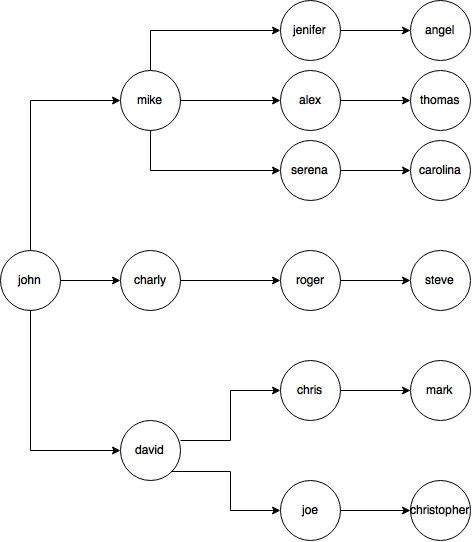
\includegraphics[width=12.5cm,height=9cm]{graph}
\\ \\To compute an \emph{answer set} representing 
a solution, invoke following command:
\\ \centerline{\texttt{shell\$ dlvhex2 --pythonplugin=extsource.py program.hex}}
where \texttt{program.hex} is \hex-program and \texttt{extsource.py} represents Python file with 
external source implementation. The output of the \dlvhex{} after solving looks as follows:


\begin{tabular}{ l r }
   $\mathit{ DLVHEX }  \mathit{ 2.4.0 } [ \mathit{ build } \mathit{ Jun } \mathit{ 23 } \mathit{ 2015 }   \mathit{ gcc } \mathit{4.8.2}]$& \\    
   $\mathit{\{personOfInterest(john), friendOfDegree(john,0,john), }$& \\
   $\mathit{invite(john), friendOfDegree(john,1,mike),}$& \\
   $\mathit{friendOfDegree(john,1,david), friendOfDegree(john,1,charly),}$ & \\
   $\mathit{invite(mike),invite(david),invite(charly)\}}$
 \end{tabular}
\\ \\
The first line shows the \dlvhex{} version, compiler version and date. The following lines
are solution of the program. Note that order in which atoms are printed does not bear any meaning. 
Same is applied to the order of sets founded. Single \emph{answer set} for this problem contain 
atoms given above. As it is expected, first atom is $\mathit{personOfInterest(john)}$ 
since $\mathit{john}$ is organizing party and program should generate set/sets of the friends 
who should be invited to the party by him. As we specified in the previous section,
we can travel at most 1 edge far from the head node. You can see from the graph that program 
can discover $\mathit{John, Mike, Charly and David}$ only since they are one edge far from the 
head node. Next three atoms are saying who are the new friends discovered and at which depth 
level. When program stop iteration through nodes due to depth constraint it starts with generating 
$\mathit{invites}$ set. It is specified by using aggregates that answer set must have four distinct $\mathit{invites}$ atoms.
In single answer set we have four $\mathit{invites}$ atoms which are $\mathit{invite(john), 
invite(mike), invite(david), invite(charly)}$. Note that this is only answer set possible 
from this program since aggregate constraint is 4 and there are only 4 distinct person that are discovered with depth level 1. If we just allow depth level to be larger there will be so many answer sets at the output since more friends will be discovered. One can just play with \emph{Depth constraint} and \emph{Aggregate constraint} to see how real output and answer sets will be affected.    

\subsection{Summary}
To conclude our quickstart, let us summarize what we did before. To solve our \emph{Social graph} problem we first provided set of facts representing instance. Second, we provided an encoding of the problem applying to any instance. With the encoding at hand, we could use \dlvhex{} to find an answer sets for the our problem. 

\section{Input Language}% Section No. 3
This section provides an overview of the input language of \dlvhex{} and provide some examples to illustrate concept. Vocabulary: terms, predicates, constants, variables and external predicates.   

\subsection{Terms and Atoms}
Terms may be integers, constants, strings and variables as well as the \enquote{\_} tokens. Constant names begin with lowercase leters and variable names begin with uppercase letters.

While a constant or string represent itself, a variable is placeholder for all variable-free terms in the language of a logic program. There is a special feature, which is called anonymous variable. The anonymous variable is denoted by ``\_" (the underscore) and is different from a usual variable. Each occurrence of \enquote{\_} represents a new and unique variable, which does not occur anywhere else in the same rule. This might be used to specify that an argument can be ignored or does not matter.

An \emph{atom} has form $\mathit{p(t_1,\dots,t_n)}$ where $p$ is a predicate name, $t_1,\dots,t_n$ are terms and $n$ $\geq$ $0$ is the arity of the predicate atom; a predicate atom $p()$ of arity 0 is likewise represented by its predicate name $p$ without parentheses. Classical atoms are: $q$, $q$ and $\neg$ $q$.

\textbf{Example 3.1.} 
Terms are:
\\ \text{Constants:} $a$, $1$, $\mathit{a1}$, $\mathit{9862}$, $\mathit{c1}$
\\ \text{Variables:} $X$, $Y$, $Z$, $\mathit{V2f}$
\\ \text{Atoms:} $a$, $b$, $\mathit{deaf}$, $\mathit{smart}$, $a$ $\leq$ $1$, $\neg$ $a$
\\ \text{Predicates:} $\mathit{parent}(X,Y)$, $\mathit{employee}(name, salary, ID, location)$
       
\subsection{Normal Programs and Integrity constraints}
\dlvhex{} is a declarative (programming) language. This means that programmer does not write an algorithm that solves some problem but instead specifies what the solution should look like, and then solves the problem and finds solution itself. Each normal logic program is constructed using \emph{facts, rules and integrity constraints}. 

\begin{tabular}{ c c c c c c r l l }

 & & & & & & \text{Fact:} & $ A_0. $ \\
 & & & & & & \text{Rule:} & $ A_0 $ :- &  $L_1$,\dots,$L_n$. \\
 & & & & & & \text{Constraint:} & :- & $ L_1$,\dots,$L_n$.   \\

\end{tabular}
\\Facts are always true. The sign \enquote{$\leftimpl$} is meant to be an implication to the left. The left side of a rule is called its \emph{head}, and right side is called its \emph{body}. The \emph{head} $A_0$ of a rule or a fact is an atom of the same syntatic form as a constant or function. In the \emph{body} of a rule or an integrity constraint, every $L_j$ for 1 $\leq$ j $\leq$ n is a literal of the form A or \emph{not} A, where A is an atom and the connective \emph{not} denotes default negation. We say that literal L is positive if it is an atom and negative otherwise. While the head atom $A_0$ of the fact must unconditionally be true, the intuitive reading of a rule corresponds to an implication: if all positive atoms in the rule body are true and negated atoms are false, then $A_0$ must be true. On the other hand, an integrity constraint is a rule that filters solution candidates, meaning that the literals in its body must not jointly be satisfied. A result of \dlvhex{} computation is called a \emph{model}. The meaning of this is clear: it is a consistent explanation(model) of the world, as far as it system can derive it. If \dlvhex{} cannot find solution then there is no model for the given problem.

\textbf{Example 3.1.} Consider the following logic program:
\begin{align*}
\mathit{ joke }.& \\
\mathit{ laugh } & \leftimpl \mathit{ joke }.
\end{align*} 
The first line here represents an \emph{atom} which is always true. The second line is a \emph{rule} and reads as \enquote{If joke is true, laugh must also be true}. Also we can read this as \enquote{from joke follows laugh}. The single \emph{model} of above program is $\{joke, laugh\}$ since they are the atoms which are true in the program. \\To explain the concept of \texttt{integrity constraints} we will consider following example:

\textbf{Example 3.2.}
\begin{align*}
&\% \text{Use edges to identify the nodes.}\\
&\mathit{node}(X) \leftimpl \mathit{edge}(X, Y). &\\
&\mathit{node}(Y) \leftimpl \mathit{edge}(X, Y). & \\
&\% \text{Guessing part.} \\
&\mathit{colored}(X, r) \text{ v } \mathit{colored}(X, g) \text{ v } \mathit{X, b} \leftimpl \mathit{node}(X). & \\
&\% \text{Checking part.} \\
&\leftimpl \mathit{edge}(X, Y), \mathit(colored)(X, C), \mathit{colored}(Y, C) & \\
&\% \text{(internal) edge definition.} \\
&\mathit{edge}(2, 4). \mathit{edge}(2, 3). \mathit{edge}(5, 5). & \\
&\mathit{edge}(4, 6). \mathit{edge}(4, 5). \mathit{edge}(5, 7). & \\
&\mathit{edge}(6, 7). &
\end{align*} 
In the first three lines one can see node declarations with variables X and Y. We concluded that X and Y are variables since they begin with uppercase letter. It says that: \enquote{If edge(X,Y) is true then node(X) is also true}. That is, it extracts the nodes from a graph specified by its edges. In the \texttt{guessing part} \dlvhex{} will list all possible models for the node(X). Each node may be coloured with either red, green or black. We did not see construction as in checking part before. It is called as \texttt{integrity constraint.} Integrity constraints in our framework specify conditions which must not become true in any model. In other words, constraints are formulations of possible inconsistencies. This mechanism is very useful in connection with disjunctive rules. The disjunctive rules serve as generators for different models and the constraints are used to select only the desired ones. Integrity constraint for this particular case will delete all those atoms from the model which does not satisfy our requirement(that there may be no edge between two nodes of equal color). Another important feature of \dlvhex{} is \texttt{default negation}. Negation is treated as "negation as failure". In other words: If an atom is not true in some model, then its negation should be considered to be true in that model. With this mechanism we can, for example, define the complementary graph of a given graph. This is the graph which has the same nodes, but of all possible edges, it has exactly those edges which do not exist in the original graph. \newpage
\begin{lstlisting}
node(X) :- edge(X,_).
node(Y) :- edge(_,Y).

comp_edge(X,Y) :- node(X), node(Y), not edge(X,Y).
\end{lstlisting}
Here \texttt{comp\_edge} describes the set of edges in the complementary graph. Such an edge must go from one node to another node (possibly the same one), and this edge must not be contained in the original edge set. Note that node(X) and node(Y) need to be included in the body in order to satisfy the following safety requirement for rules: Variables, which occur in a negated literal, must also occur in a positive literal in the body.

\subsection{Classical Negation}
\dlvhex{} supports two kinds of negation. Here we will emphasize difference between explicitly expressing falseness of an atom and having it done by \texttt{Complete World Assumption}. The connective \texttt{not} expresses default negation, i.e. a literal \texttt{not A} is assumed to hold unless atom A is derived to be true. In contrast, the classical (or strong) negation of an atom holds only if it can be derived. In other words if there is no evidence that an atom is true, it is considered to be false. Classical negation, indicated by symbol \enquote{-}, is permitted in from of an atoms. The semantic relationship between A and -A is simply that they must not jointly hold. 
\\ \textbf{Example 3.3.}
\\ Imagine a simple situation, in which and agent has to cross a railroad. The agent should cross it if there is no train approaching. With this description, one might specify the following program:
\begin{lstlisting}
 cross_railroad :- not train_approaches.
\end{lstlisting}
The following program has the model \textit{cross} because $train\_approaches$ is assumed to be false(as it being true is not stated anywhere). This kind of negation is called negation as failure.\\The next program uses so-called true or classical negation. Since \textit{$-train\_approaches$} is not known to be true, the following program has only an empty model.
\begin{lstlisting}
 cross_railroad :- -train_approaches.
\end{lstlisting}
The difference between the two kinds of negation is quite important: In the first example, we cross the railroad track if we have no information on any trains approaching, which is quite dangerous, while in the second example, we only cross if we know for sure that no train comes. It is important to note that classical negation is stronger than negation as finite failure. If something is true via true negation, it is always also true if negated by negation as failure.

\subsection{Disjunction}
Disjunctive logic programs permit the connective 'v' between atoms in rule heads. \\
\begin{tabular}{ c c c c c c r l l}
 & & & & & & \texttt{Fact:} & $A_0$ v \dots v $A_m$ \\
 & & & & & & \texttt{Rule:} & $A_0$ v \dots v $A_m$ :- $L_1,\dots,L_n. $ \\
 \end{tabular}
\\ The \texttt{head} $A_0$ of a rule or a fact is an atom of the same syntatic form as a constant or function. In the \texttt{body} of a rule or an integrity constraint, every $L_j$ for 1 $\leq$ j $\leq$ n is a literal of the form A or \texttt{not} A, where A is an atom and the connective \texttt{not} denotes default negation. We say that literal L is positive if it is an atom and negative otherwise. While the head atom $A_0$ of the fact must unconditionally be true, the intuitive reading of a rule corresponds to an implication: if all positive atoms in the rule body are true and negated atoms are false, then $A_0$ must be true. A \texttt{disjunctive head} holds if at least one of its atomes is true. In a simple disjunctive program \texttt{a v b.} we have the two answer sets \{a\} and \{b\}.
\\ \textbf{Example 3.4.}
\begin{lstlisting}
left_arm_broken v right_arm_broken.
can_write :- left_arm_broken.
be_angry :- can_write
\end{lstlisting}
Suppose you have met a friend recently and know that he had one of his arms broken, but do not know which one. Now suppose we did not receive a greeting card for your birthday and wonder if you should be angry on him or he just could not write because his right hand is broken. In example, \dlvhex{} will generate two possible explanations. The first rule is called a disjunctive rule; the v is read as \enquote{or} and the whole rule is read as \enquote{For sure, either the left or the right arm is broken.} Without being sure which arm is broken \dlvhex{} will evaluate the program and produce the two models \texttt{$\{left\_arm\_broken, can\_write, be\_angry$\}} and \texttt{$\{right\_arm\_broken$\}}.  

\subsection{Built-in Arithmetic Functions}
Beside integers (constant arithmetic functions), written as sequence of digits 0 \dots 9, \dlvhex{} supports other types of arithmetic functions. We are using the following operators for those functions: + (addition), - (subtraction), * (multiplication), / (integer division). \\ \textbf{Example 3.5.}
\begin{lstlisting}
% This example demonstrates usage of built-in arithmetic functions
a(6).
b(2).

c(X,Y,XX) :- a(X), b(Y),+(X, Y, XX).
d(X,Y,XX) :- a(X), b(Y),-(X, Y, XX).
e(X,Y,XX) :- a(X), b(Y),*(X, Y, XX).
f(X,Y,XX) :- a(X), b(Y),/(X, Y, XX).
\end{lstlisting}
The single answer set for the example above is: \\ \texttt{\{a(6),b(2),e(6,2,12),f(6,2,3),c(6,2,8),d(6,2,4)\}}
\\Except \texttt{prefix notation} we can also use \texttt{infix notation} to use built-in arithmetic functions in \dlvhex{}. Instead of writing +(X, Y, XX) alternatively we can write it as XX=X+Y. 
     
\subsection{Built-in Comparison Predicates}
\dlvhex{} feature a total order among variable-free terms using built-in predicates == (equal), != (not equal), $<$ (less than), $\leq$ (less than or equal), $>$ (greater than) and $\geq$ (greater than or equal). All kinds of constants (symbols and integers) may be compared against each other freely. If two integers are compared, the semantics are as expected. All other comparisons are just guaranteed to impose a fixed ordering over all constants. The application of comparison literals to integers is illustrated by the following example.
\\ \textbf{Example 3.6.}
\begin{lstlisting}
% This example demonstrates usage of built-in 
% comparison predicates

a(1).
a(2).
b(1).

c(X,Y) :- a(X), b(Y), X <> Y.
d(X,Y) :- a(X), b(Y), X != Y.
e(X,Y) :- a(X), b(Y), X < Y.
f(X,Y) :- a(X), b(Y), X > Y.
g(X,Y) :- a(X), b(Y), X <= Y.
h(X,Y) :- a(X), b(Y), X >= Y.
i(X,Y) :- a(X), b(Y), Y == 1.
\end{lstlisting}
The single answer set for the example above is:\\ \texttt{\{a(1),a(2),b(1),i(1,1),i(2,1),c(2,1),d(2,1),f(2,1),g(1,1),h(1,1),h(2,1)\}}


\subsection{Conditions and Conditional Literals}
A \textit{conditional literal} is of the form \\ \centerline{$L_0:L_1,\dots,L_n$} where every \textit{$L_j$ for 0 $\leq$ j $\leq$ n} is a literal, $L_1,\dots,L_n$ is called \textit{condition}, and \enquote{:} resembles mathematical set notation. Whenever \texttt{n = 0}, it is a regular literal and we denote it usually by $L_0$.
\\For example, the rule \\ \texttt{a :- b : c.} \\yields \texttt{a} whenever either \texttt{c} is false (whether \texttt{b} holds or not) or both \texttt{b} and \texttt{c} are true \cite{pott}. \\Together  with variables, conditions allow for specifying collections of expressions within a single rule or aggregate. This is particularly useful for encoding conjunctions(or disjunctions) over arbitrarily many ground atoms as well as for the compact representation of aggregates. 
\\ \textbf{Example 3.7.}
\begin{lstlisting}
% This example demonstrates usage of conditions in rule's 
% head and body

person(jane). person(john).
day(mon). day(tue). day(wed). day(thu). day(fri).
available(jane) :- not on(fri).
available(john) :- not on(mon), not on(wed).
meet :- available(X) : person(X).
on(X) : day(X) :- meet.
\end{lstlisting}  
We have used conditions in last two lines of the code. The conjunction in the body of line 5 is obtained by replacing X in \texttt{available(X)} with all ground terms \texttt{t} such that \texttt{person(t)} holds, namely, with t=jane and t=john. The condition for the last line is contained in the head of rule. It turns into disjunction over all ground instances of \texttt{on(X)} such that X is substituted by terms t for which \texttt{day(t)} holds. Any variable occurring within a condition does not count as a positive occurrence outside the condition in the sense of safety. A variable X in an aggregate-free rule is safe if at least one of the following conditions is satisfied:\\-X occurs in a positive standard predicate in the body of the rule;\\-X occurs in a true negated standard predicate in the body of the rule;\\-X occurs in the last argument of an arithmetic predicate A and all other arguments of A are safe. \\ \\A rule is safe if all its variables are safe. Variables occurring in atoms not subject to any conditions are global. Each variable within an atom in front of a condition must be global or have a positive occurrence on the right hand-side of the condition. During grounding, the instantiation of global variables take precedence over non-global ones, that is, the former are instantiated before the latter.As a consequence, variables that occur globally are substituted by terms before a condition is further evaluated \cite{pott}.    
\subsection{Aggregates}
Aggregates allow to express properties over set of elements. DLV and \hex{}-programs with aggregates often allow clean and concise problem encodings by minimizing the use of auxiliary predicates and recursive programs, and help the programmers to depict problems in a more natural way. For instance, we may state that the sum of a semester's course credits must be at least 20, or that the sum of shopping items must not exceed 30 Euros. We can say that an aggregate is a function on a set of tuples that are normally subject to conditions. By comparing an aggregated value with given values, we can extract a truth value from an aggregate's evaluation, thus obtaining an aggregate atom 
They can occur in the bodies of rule and constraints, possibly negated using negation-as-failure. \\ \texttt{Body Aggregates} The form of an \texttt{aggregate atom} occuring in a rule body is as follows:\\ \centerline{$s_1 \prec_1 \alpha \{ t_1:L_1;...;t_n:L_n\} \prec_2 s_2$} 
\\ Here, all \texttt{$t_i$} and \texttt{$L_i$}, forming \texttt{aggregate elements}, are non-empty tuples of terms and literals, respectively. $\alpha$ is the name of some function that is applied to the term tupples \texttt{$t_i$} that remain after evaluating the conditions expressed by $L_i$. Finally,  the result of applying $\alpha$ is compared by means of the comparison predicates $\prec_1 or \prec_2$ to the terms $s_1$ and $s_2$ respectively. \#count, \#sum, \#times, \#min, and \#max are called aggregate functions, and \dlvhex{} currently supports exactly these five. An aggregate function is applied over a set and returns a numeric value.
\\ \textbf{Example 3.8.}
\begin{lstlisting}
% This example demonstrates usage of aggregate functions:
% Each employee is is represented by a fact of the form 
% emp(ID,NAME,SALARY)

emp(1,goofie,1250).
emp(2,willy,700).
emp(3,woody,750).
emp(4,jerry,900).
emp(5,tom,1050).
\end{lstlisting}
Intuitively the symbolic set appearing in the aggregate predicate consists of two ground predicates: \\ \centerline{$\{<1,over1000(1,1250)>,<5,over1000(5,1050)>\}$}
\\which are both true w.r.t. the unique model of the whole program, hence \\ \centerline{$ \#count\{over1000(1,1250),over1000(5,1050)\}$} \\returns 2 as output of aggregate function and outputs:\\ \texttt{(1,goofie,1250),emp(2,willy,700),emp(3,woody,750),emp(4,jerry,900),\\emp(5,tom,1050),over1000(1,1250),over1000(5,1050),over1000nr(2)}
\\as a result of the program.
The aggregate function \texttt{\#count} returns the cardinality of the symbolic set to which it is applied. We want to count how many employees of the company earn more than 1000. 
\begin{lstlisting}
over1000(I,S) :- emp(I,N,S), S > 1000.
over1000nr(X) :- #count{I : over1000(I,W)} = X, #int(X).
\end{lstlisting}
\bigskip Let $f(S)$ be an aggregate function. A variable, X, is a \texttt{local variable} to $f(S)$ if and only if X appears in S and X does not appear in any aggregate function that is outer to $f(S)$. Aggregate function \texttt{\#sum} returns the sum of the first local variable to be aggregated over in the symbolic set. Suppose we want to know how much the Cartoon Co. spends on salaries.
\begin{lstlisting}
salaryTotal(X) :- #sum{S,I : emp(I,N,S)} = X.
\end{lstlisting}
The symbolic set here consists of 5 elements, namely all of the facts stored in the database of the employees. The aggregate function applied to the given set returns the sum of the salaries of all the employees, the output thus is:
{salaryTotal(4650)}. \textbf{\#times} is similar to \#sum, but computes the product of the first local variable to be aggregated over in the symbolic set. When applied over the empty set, \#times returns 1.
\bigskip \\The aggregate function \textbf{\#min} returns the minimum value of the first local variable to be aggregated over in the symbolic set. The following simple program then returns the lowest income among all employees.
\begin{lstlisting}
lowest(X) :- #min{S : emp(I,N,S)} = X.
\end{lstlisting}
The aggregate function applied to the given set returns the minimum salary among of all the employees, the output thus is:
{lowest(700)}
\bigskip \\ The aggregate function \textbf{\#max} returns the maximum value of the first local variable to be aggregated over in the symbolic set. The following program computes the maximum income earned in the company
\begin{lstlisting}
highest(X) :- #max{S : emp(I,N,S)} = X.
\end{lstlisting}
and it outputs $\{highest(1250)\}$ as a highest income in the company.

\subsection{Optimization}
Introducing \texttt{weak constraints} into \hex-programs allows us to formulate several optimization problems in an easy and natural way. These weak constraints are adopted from \texttt{DLV}. While standard constraints (integrity constraints, strong constraints) always have to be satisfied, weak constraints should be satisfied if it is possible, but their violation does not \enquote{local variable} the models.\\The answer sets of a program P with a set W of weak constraints are those answer sets of P which minimize the violation of weak constraints respecting their weights and levels. They are called best models of (P,W). Note that a program may have several best models.\\ Weak constraints can be weighted according to their importance (the higher the weight, the more important the constraint). In the presence of weights, best models minimize the sum of the weights of the violated weak constraints. Weak constraints can also be prioritized. Under prioritization, the semantics minimizes the violation of the constraints of the highest priority level first; then the lower priority levels are considered one after the other in descending order. Syntactically, weak constraints are specified as follows. \\ \centerline{$:~ Conj. [Weight:Level]$} \\ where Conj is a conjunction of (possibly negated) literals, and both Weight and Level are positive integers. Weights and priority levels are allowed to be variables, provided that these variables also appear in a positive literal in Conj.
The following program, computes the minimum spanning trees of a weighed directed graph.
\\ \textbf{Example 3.9.}
\begin{lstlisting}
root(a).
node(a). node(b). node(c). node(d). node(e).
edge(a,b,4). edge(a,c,3). edge(c,b,2). edge(c,d,3). 
edge(b,e,4). edge(d,e,5).

in_tree(X,Y,C) v out_tree(X,Y) :- edge(X,Y,C), reached(X).
:- root(X), in_tree(_,X,C).
:- in_tree(X,Y,C), in_tree(Z,Y,C), X != Z.

reached(X):- root(X).
reached(Y):- reached(X), in_tree(X,Y,C).
:- node(X), not reached(X).

: in_tree(X,Y,C). [C:1]
\end{lstlisting}
Best model: \texttt{\{reached(a), out\_tree(a,b), in\_tree(a,c,3), reached(b), reached(c), in\_tree(b,e,4), in\_tree(c,b,2), in\_tree(c,d,3), reached(e), reached(d), out\_tree(d,e)\}}
\\Cost ([Weight:Level]): $<[12:1]>$
\\Finally, we show an example where both weights and priorities are specified. This example and some others are taken from the DLV-User Manual \cite{dlvum}. Consider the problem of assigning a given set of employees to two projects. As a minor desideratum, we wish that members of the same group already know each other. Higher level constraints ask each group to be heterogeneous as far as skills are concerned, and require that people married with one another do not work in the same group.
\\ \textbf{Example 3.10.}
\begin{lstlisting}
% This example specify both weights and priorities
employee(a). employee(b). employee(c). employee(d). employee(e).
know(a,b). know(b,c). know(c,d). know(d,e).
same_skill(a,b).
married(c,d).

member(X,p1) v member(X,p2) :- employee(X).
:~ member(X,P), member(Y,P), X != Y, not know(X,Y). [1:1]
:~ member(X,P), member(Y,P), X != Y, married(X,Y). [1:2]
:~ member(X,P), member(Y,P), X != Y, same_skill(X,Y). [1:2] 
\end{lstlisting}
This program has two best models:
\\ \texttt{Best model:}\{member(a,p2), member(b,p1), member(c,p1), member(d,p2), member(e,p2)\}
\\Cost ([Weight:Level]): $<[6:1],[0:2]>$
\\ \\ \texttt{Best model:}\{member(a,p1), member(b,p2), member(c,p2), member(d,p1), member(e,p1)\}
\\Cost ([Weight:Level]): $<[6:1],[0:2]>$

\subsection{High-order}
Now we introduce the most specific feature of \dlvhex{} compared to other ASP solvers. \hex{}-programs are nonmonotonic logic programs admitting \texttt{high-order atoms} as well as \texttt{external atoms}, and we extend the well known answer-set semantics to this class of programs. Advantage of using external atoms is increasing software interoperability. \\Let $C$,$X$, and $G$ be mutually disjoint sets whose elements are called \texttt{constant names, variable names,} and \texttt{external predicate names,} respectively. Unless explicitly specified, elements from \texttt{$X$} are denoted with first letter in upper case, while elements from \texttt{$G$} are prefixe with \enquote{\&}. 
We note that the constant names serve both as individual and predicate names. Elements from \texttt{$C$} $\cup$ \texttt{$X$} are called \texttt{terms}. \\ \\A high-order atom allows to quantify values over predicate names, and to freely exchange predicate symbols with constant symbols, like in the rule\\ \centerline{\\$C(X) \leftarrow \textit{subclassOf(D,C),D(X)}$}
A \textit{high-order atom} is a tuple ($Y_0, Y_1,\dots,Y_n$), where $Y_0, Y_1,\dots,Y_n$ are terms; $ n \ge 0$ is the \textit{arity} of the atom. Intuiitively, $Y_0$ is the predicate name, and we thus also use the more familiar notation $Y_0(Y_1,\dots,Y_n)$. The atom is \textit{ordinary}, if $Y_0$ is a constant. For example, \textit{(x,rdf:type,c),node(X), and D(a,b),} are atoms;the first two are ordinary atoms. An \textit{external atom} is of the form \\ \centerline{ \&g[$Y_1,\dots,Y_n$]($X_1,\dots,X_m$),} \\where $Y_1,\dots,Y_n$ and $X_1,\dots,X_m$ are the two lists of terms (called \textit{input} and \textit{output} lists, respectively), and \&g $\in$ \textit{G} is an external predicate name. We assume that \&g has fixed lengths \texttt{in($\&g$)} = n and \texttt{out($\&g$)} = m for input and output lists, respectively. Intuitively, an external atom provides a way for deciding the truth value of an output tuple depending on the extension of a set of input predicates.       
\\To understand concept better we are providing example which show how we can get use of external atoms in ordinary ASP.

\subsection{External Atoms}
Through external atoms, \hex{}-programs can communicate with other sources of computation; this can be used to model extensions of ASP.  
An \texttt{external atom} facilitates to determine the truth value of an atom through an external source of computation. For instance, the rule \\ \centerline{ \textit{$reached(X) \leftarrow \&reach[edge,a](X)$}}
\\computes the predicate \textit{reached} taking values from the predicate $\&reach$, which computes via \textit{$\&reach[edge,a](X)$} all the reachable nodes in the graph in the graph \textit{edge} from node \textit{a}, delegating this task to an external computational source (e.g., an external deduction system, an execution library, etc.). 

\textbf{\\Example 3.11.}
\\ \lstinputlisting{introductiontohex.hex}     
This \hex{}-program  which works with constant input parameters  to external sources. For each system, it concatenates the string \enquote{hello} and a system name using \texttt{$\&$concat} external source. At output we have the answer set like:\\ \{ \texttt{sayhello(hellodlvhex), sayhello(helloclasp)} \}. 
\\Second part of the program works with predicate input parameters. It first define two different sets and then computes \texttt{set1} minus \texttt{set2} using \texttt{$\&$setdiff} external source.




\newpage
\section{References}
\begin{thebibliography}{1}
\bibitem{extatoms} Thomas Eiter, Micheal Fink, Thomas Krennwallner, Christoph Redl {\em Conflict-driven ASP Solving with External Sources} 2003   
  
\bibitem{ref} Francesco Calimeri, Wolfgang Faber, Martin Gebser, Giovambattista Ianni, Roland Kaminski, Thomas Krennwallner, Nicola leone, Francesco Ricca, Torsten Schaub {\em ASP-Core-2 Input Language} 2013.

\bibitem{licnc} GNU Lesser General Public License. Free Software Foundation, Inc. https://www.gnu.org/copyleft/lesser.html 

\bibitem{onlinedemo}dlvhex. Vienna University of Technology. http://www.kr.tuwien.ac.at/research/systems/dlvhex/demo.php 

\bibitem{git}Software for HEX-Programs. GitHub. https://github.com/hexhex/ 

\bibitem{sourceforge}DLVHEX solver for HEX-programs-  Browse Files at SourceForge.net. Sourceforge.net. http://sourceforge.net/projects/dlvhex/files/

\bibitem{prebuilt}KBS-ASP systems. Thomas Krenwallner. http://www.kr.tuwien.ac.at/staff/tkren/deb.html

\bibitem{boost}Boost C++ Libraries. Boost.org. http://www.boost.org/

\bibitem{hexhex}dlvhex. GitHub. https://github.com/hexhex/core

\bibitem{script}Web location for script

\bibitem{extatoms2}Thomas Eiter, Giovamattista Ianni, Roman Schindlauer and hans Tompits {\em A Uniform Integration of Higher-Order Reasoning and External Evaluations in Answer-Set Programming} 


\bibitem{pott}Martin Gebser, Roland Kaminski, Benjamin Kaufmann, Marius Lindauer, Max Ostrowski, Javier Romero, Trosten Schaub and Sven Thiele {\em Pottasco User Guide}

\bibitem{dlvum}Robert Bihlmeyer, Wolfgang Faber, Giuseppe Ielpa, Vincezino Lio and Gerald Pfeifer {\em DLV-User Manual} 
      
 
 \end{thebibliography} 



\end{document}

